\begin{activity} \label{A:10.1.1} Consider the function $f$, defined by
  $$
  f(x,y) = \frac{y}{\sqrt{x^2+y^2}},
  $$ 
  whose graph is shown below in
  Figure \ref{F:10.1.disc.2}

  \begin{figure}[ht]
    \begin{center}
      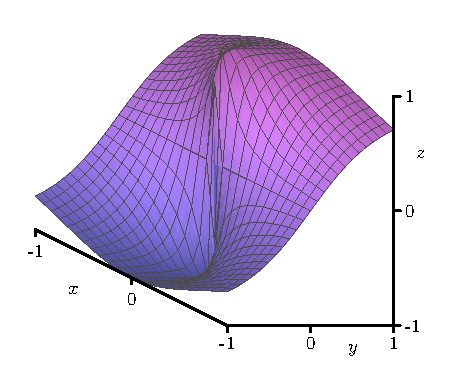
\includegraphics{figures/fig_10_1_disc_2.eps}
      \caption{The graph of $f(x,y) = \frac{y}{\sqrt{x^2+y^2}}$.}
      \label{F:10.1.disc.2}
    \end{center}
  \end{figure}

      
  \ba
\item Is $f$ defined at the point $(0,0)$?  What, if anything, does
  this say about whether $f$ has a limit at the point $(0,0)$? 

\item Values of $f$ (to three decimal places) at several points close to
  $(0,0)$ are shown in the table below. 
  \begin{center}
    \begin{tabular}{|r||c|c|c|c|c|}
      \hline
      $x\backslash y$ & -1 & -0.1 & 0 & 0.1 & 1 \\       \hhline{|=|=|=|=|=|=|}
      $-1$ & $-0.707$ & --- & 0 & ---  & $0.707$ \\       \hline
      $-0.1$ & --- & $-0.707$ & 0 & $0.707$ &  --- \\       \hline
      0 &$-1$ &$-1$ &--- &1 &1 \\       \hline
      0.1 & --- &$-0.707$ &0 &$0.707$ & --- \\       \hline
      1 &$-0.707$ &--- &0 &--- & $0.707$\\       \hline
    \end{tabular}
  \end{center}
%   \begin{center}
%    \begin{tabular}{|c||c|c|c|c|c|}
%      \hline
%      $x\backslash y$ & -1 & -0.1 & 0 & 0.1 & 1 \\
%      \hhline{|=|=|=|=|=|=|}
%      $-1$ & \hspace*{0.5in} & --- & \hspace*{0.5in} & ---
%      & \hspace*{0.5in} \\ 
%      \hline
%      $-0.1$ & --- & \hspace*{0.5in} & & \hspace*{0.5in} &  --- \\
%      \hline
%      0 & & &--- & & \\
%      \hline
%      0.1 & --- & & & & --- \\
%      \hline
%      1 & &--- & &--- & \\
%      \hline
%    \end{tabular}
%  \end{center}
  
  Based on these calculations, state whether $f$ has a limit at
  $(0,0)$ and give an argument supporting your statement. (Hint: The blank spaces in the table are there to help you see the patterns.)
	
\item Now let's consider what happens if we restrict our attention to
  the $x$-axis;  that is, consider what happens when $y = 0$.  
  What is the behavior of $f(x,0)$ as $x \to 0$?  If we approach
  $(0,0)$ by moving along the $x$-axis, what value do we find as the
  limit?  

\item What is the behavior of $f$ along the line $y=x$ when $x> 0$;  that
  is, what is the value of $f(x,x)$ when $x>0$?  If we approach $(0,0)$ by moving
  along the line $y=x$ in the first quadrant (thus considering $f(x,x)$ as $x \to 0$, what value do we find as the limit?

\item In general, if $\lim_{(x,y)\to(0,0)}f(x,y) = L$, then $f(x,y)$ approaches
  $L$ as $(x,y)$ approaches $(0,0)$, regardless of the path we take in letting $(x,y) \to (0,0)$.   Explain what the last two parts
  of this activity imply about the existence of $\lim_{(x,y)\to(0,0)} f(x,y)$.

\item Shown below in Figure \ref{F:10.1.limit_contour_2} is a set of
  contour lines of the function $f$.  What is the behavior of
  $f(x,y)$ as $(x,y)$ approaches $(0,0)$ along any straight line?  
  How does this observation reinforce your conclusion about the
  existence of $\lim_{(x,y)\to(0,0)}f(x,y)$ from the previous part of
  this activity? (Hint: Use the fact that a non-vertical line has equation $y=mx$ for some constant $m$.)

  \begin{figure}[ht]
    \begin{center}
      
\includegraphics{figures/fig_10_1_limit_contour_2.eps}
      \caption{Contour lines of $f(x,y) = \frac{y}{\sqrt{x^2+y^2}}$.}
      \label{F:10.1.limit_contour_2}
    \end{center}
  \end{figure}

	
	
	\ea
\end{activity}

\begin{activitySolution}
\ba
\item Since the denominator is 0 when $(x,y) = (0,0)$, the function $f$ is not defined at the origin. However, a function can have a limit at a point where it is undefined, so this information does not determine if $f$ has a limit at $(0,0)$ or not.
\item It looks as though the values of $f$ are approaching different numbers (e.g., $-1$, $-0.707$, $0.707$, $1$) as $(x,y)$ nears $(0,0)$. The function $f$ will have a limit at the point $(0,0)$ if all of the values of the function become arbitrarily close to one fixed number as $(x,y)$ gets as close to $(0,0)$ as we want. Since the values of $f$ do not approach a single fixed number as $(x,y)$ gets close to $(0,0)$, we should conclude that $f$ does not have a limit at $(0,0)$.   
\item When $y=0$ we have $f(x,y) = f(x,0) = 0$ as indicated in the table. So $\lim_{x \to 0} f(x,0) = 0$. 
\item When $x > 0$ we have $f(x,y) = f(x,x) = \frac{x}{\sqrt{2x^2}} = \frac{1}{\sqrt{2}}$. So  $\lim_{x \to 0} f(x,x) = \frac{1}{\sqrt{2}} \approx 0.707$ as illustrated in the table.
\item The fact that $f(x,y)$ gets arbitrarily close to $0$ as $(x,0)$ gets as close to $(0,0)$ as we want and the fact that $f(x,y)$ gets arbitrarily close to $\frac{1}{\sqrt{2}}$ as $(x,x)$ gets as close to $(0,0)$ as we want shows that there is no fixed number $L$ that all of the values of $f(x,y)$ approach as $(x,y)$ gets close to $(0,0)$. So $f$ does not have a limit at $(0,0)$. 
\item When $y=mx$ we have $f(x,y) = f(x,mx) = \frac{mx}{(1+m^2)x^2}$. If $x>0$, then $f(x,mx) = \frac{m}{1+m^2}$ and if $x < 0$, then $f(x,mx) = -\frac{m}{1+m^2}$. In either case, the values $f(x,mx)$ do not all approach the same number $L$ as $x$ gets arbitrarily close to $0$. In other words, $f$ has different limits along different paths that contain the origin. 
\ea
\end{activitySolution}

\aftera

